\scanpage{43}
\margin{Notion \uline{loc.} \uline{\unsure{triviale}}\unsure{?}}

[\uline{Corollaire} $P$ fibré projectif $\unsure{\Longleftrightarrow|\Longrightarrow}$ $P$ \unsure{adm} loc. une section \inserted{(i.e. est loc. \unsure{trivial})\deleted{\unsure{fibré projectif}}}, et une certaine obstruction dans $H^2(S,\underline{O}_S^*)$ est nulle\ldots]
\margin{en conséquence.}

[\uline{Corollaire} Si $S$ régulier, $P$ fibré projectif ssi il est loc. trivial, ou encore ssi ses fibres génériques le sont.
\margin{\unsure{peut être avec prop 2}}

Autre façon de procéder, valable si $S$ est \uline{strictement \inserted{loc} factoriel} [i.e. tout \uline{schéma} étale dessus est \inserted{loc} factoriel] ----
\figure{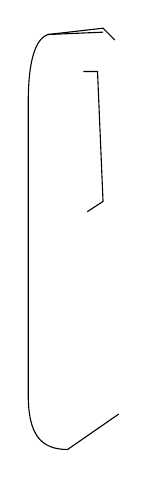
\begin{tikzpicture}[x=1cm,y=1cm]
\draw (0.4,5.1) -- (0.25,5.25) -- (-0.45,5.17) .. controls (-0.65,5.1) and (-0.7,4.7) .. (-0.7,4.3) -- (-0.7,0.6) .. controls (-0.7,0.1) and (-0.55,-0.1) .. (-0.2,-0.1) -- (0.45,0.35);
\draw (-0.45,5.17) -- (0.25,5.2);
\draw (0,4.7) -- (0.18,4.7) -- (0.25,3.05) -- (0.05,2.92);
\end{tikzpicture}}

\uline{Corollaire} \unsure{locale isotrivialité}.
\figure{\begin{tikzpicture}\draw (0,0) .. controls (4,0.15) and (9,0.55) .. (13,0.75);\end{tikzpicture}}

b) \uline{Déf} \uline{Système linéaire} \inserted{\uline{de div. sur} $X/S$}, \uline{paramétré} \uline{par un schéma} $\check{P}/S$ : c'est loc fppf un syst. lin. de div. paramétré par un fibré projectif.
\margin{[$X\to S$ \unsure{fid\textsuperscript{t}} plat loc prés. finie]}
\deleted{Système linéaire}

\deleted{\unsure{Indiquer que}}
Indiquer que $P/S$ est un schéma de Brauer-Séveri.
\margin{\uline{Système linéaire} (tt court).}

classe d'équivalence .....
\mspage{42}
